\begin{frame}\frametitle{\vspace*{0.5cm}I aim to further our understanding of the relevant fluid mechanics}
  \begin{figure}
    \centering%
    \hfill%
    \begin{tikzpicture}%
      \node[anchor=south west,inner sep=0] (image) at (0,0) {%
        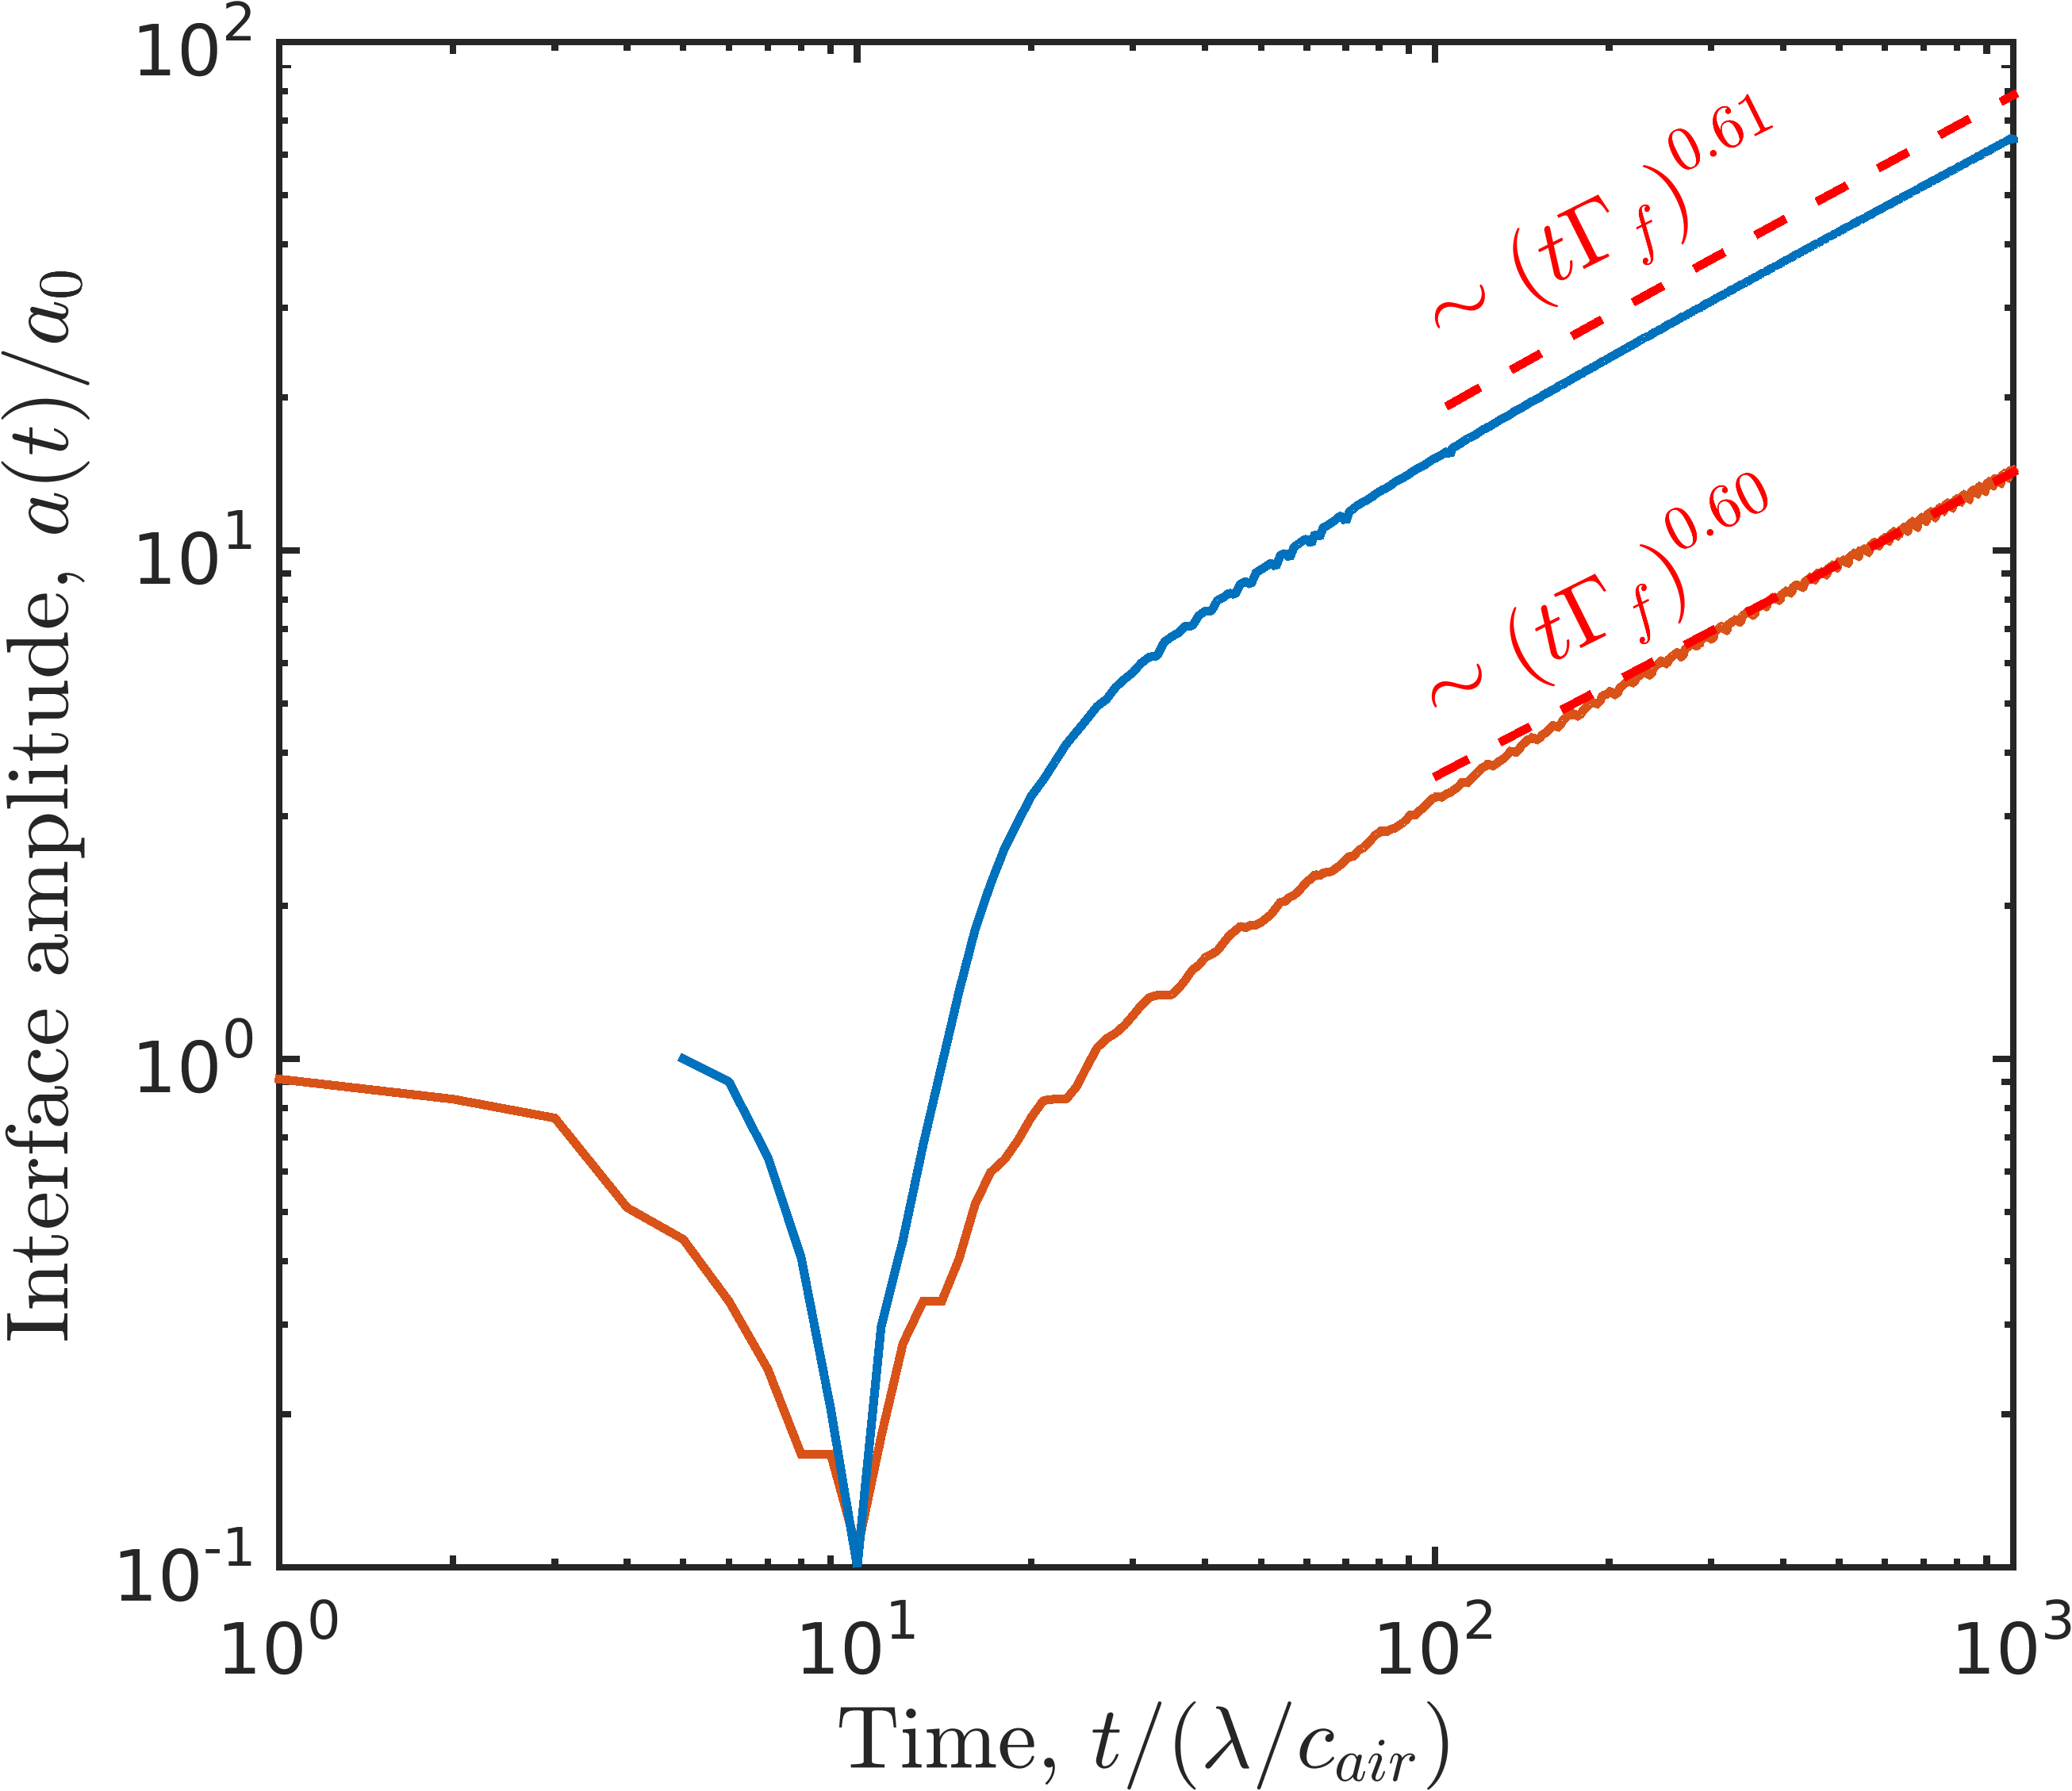
\includegraphics[height=0.45\textheight]{../figs/lung_figs/interface_multi-amp_loglog_roe_t1000}%
      };%
      \begin{scope}[x={(image.south east)},y={(image.north west)}]%
        \node[font=\footnotesize,right] at (0.32,0.7){ $10$ MPa};%
        \node[font=\footnotesize,right] at (0.55,0.4){ $5$ MPa};%
      \end{scope}%  
    \end{tikzpicture}%
    \hfill%
    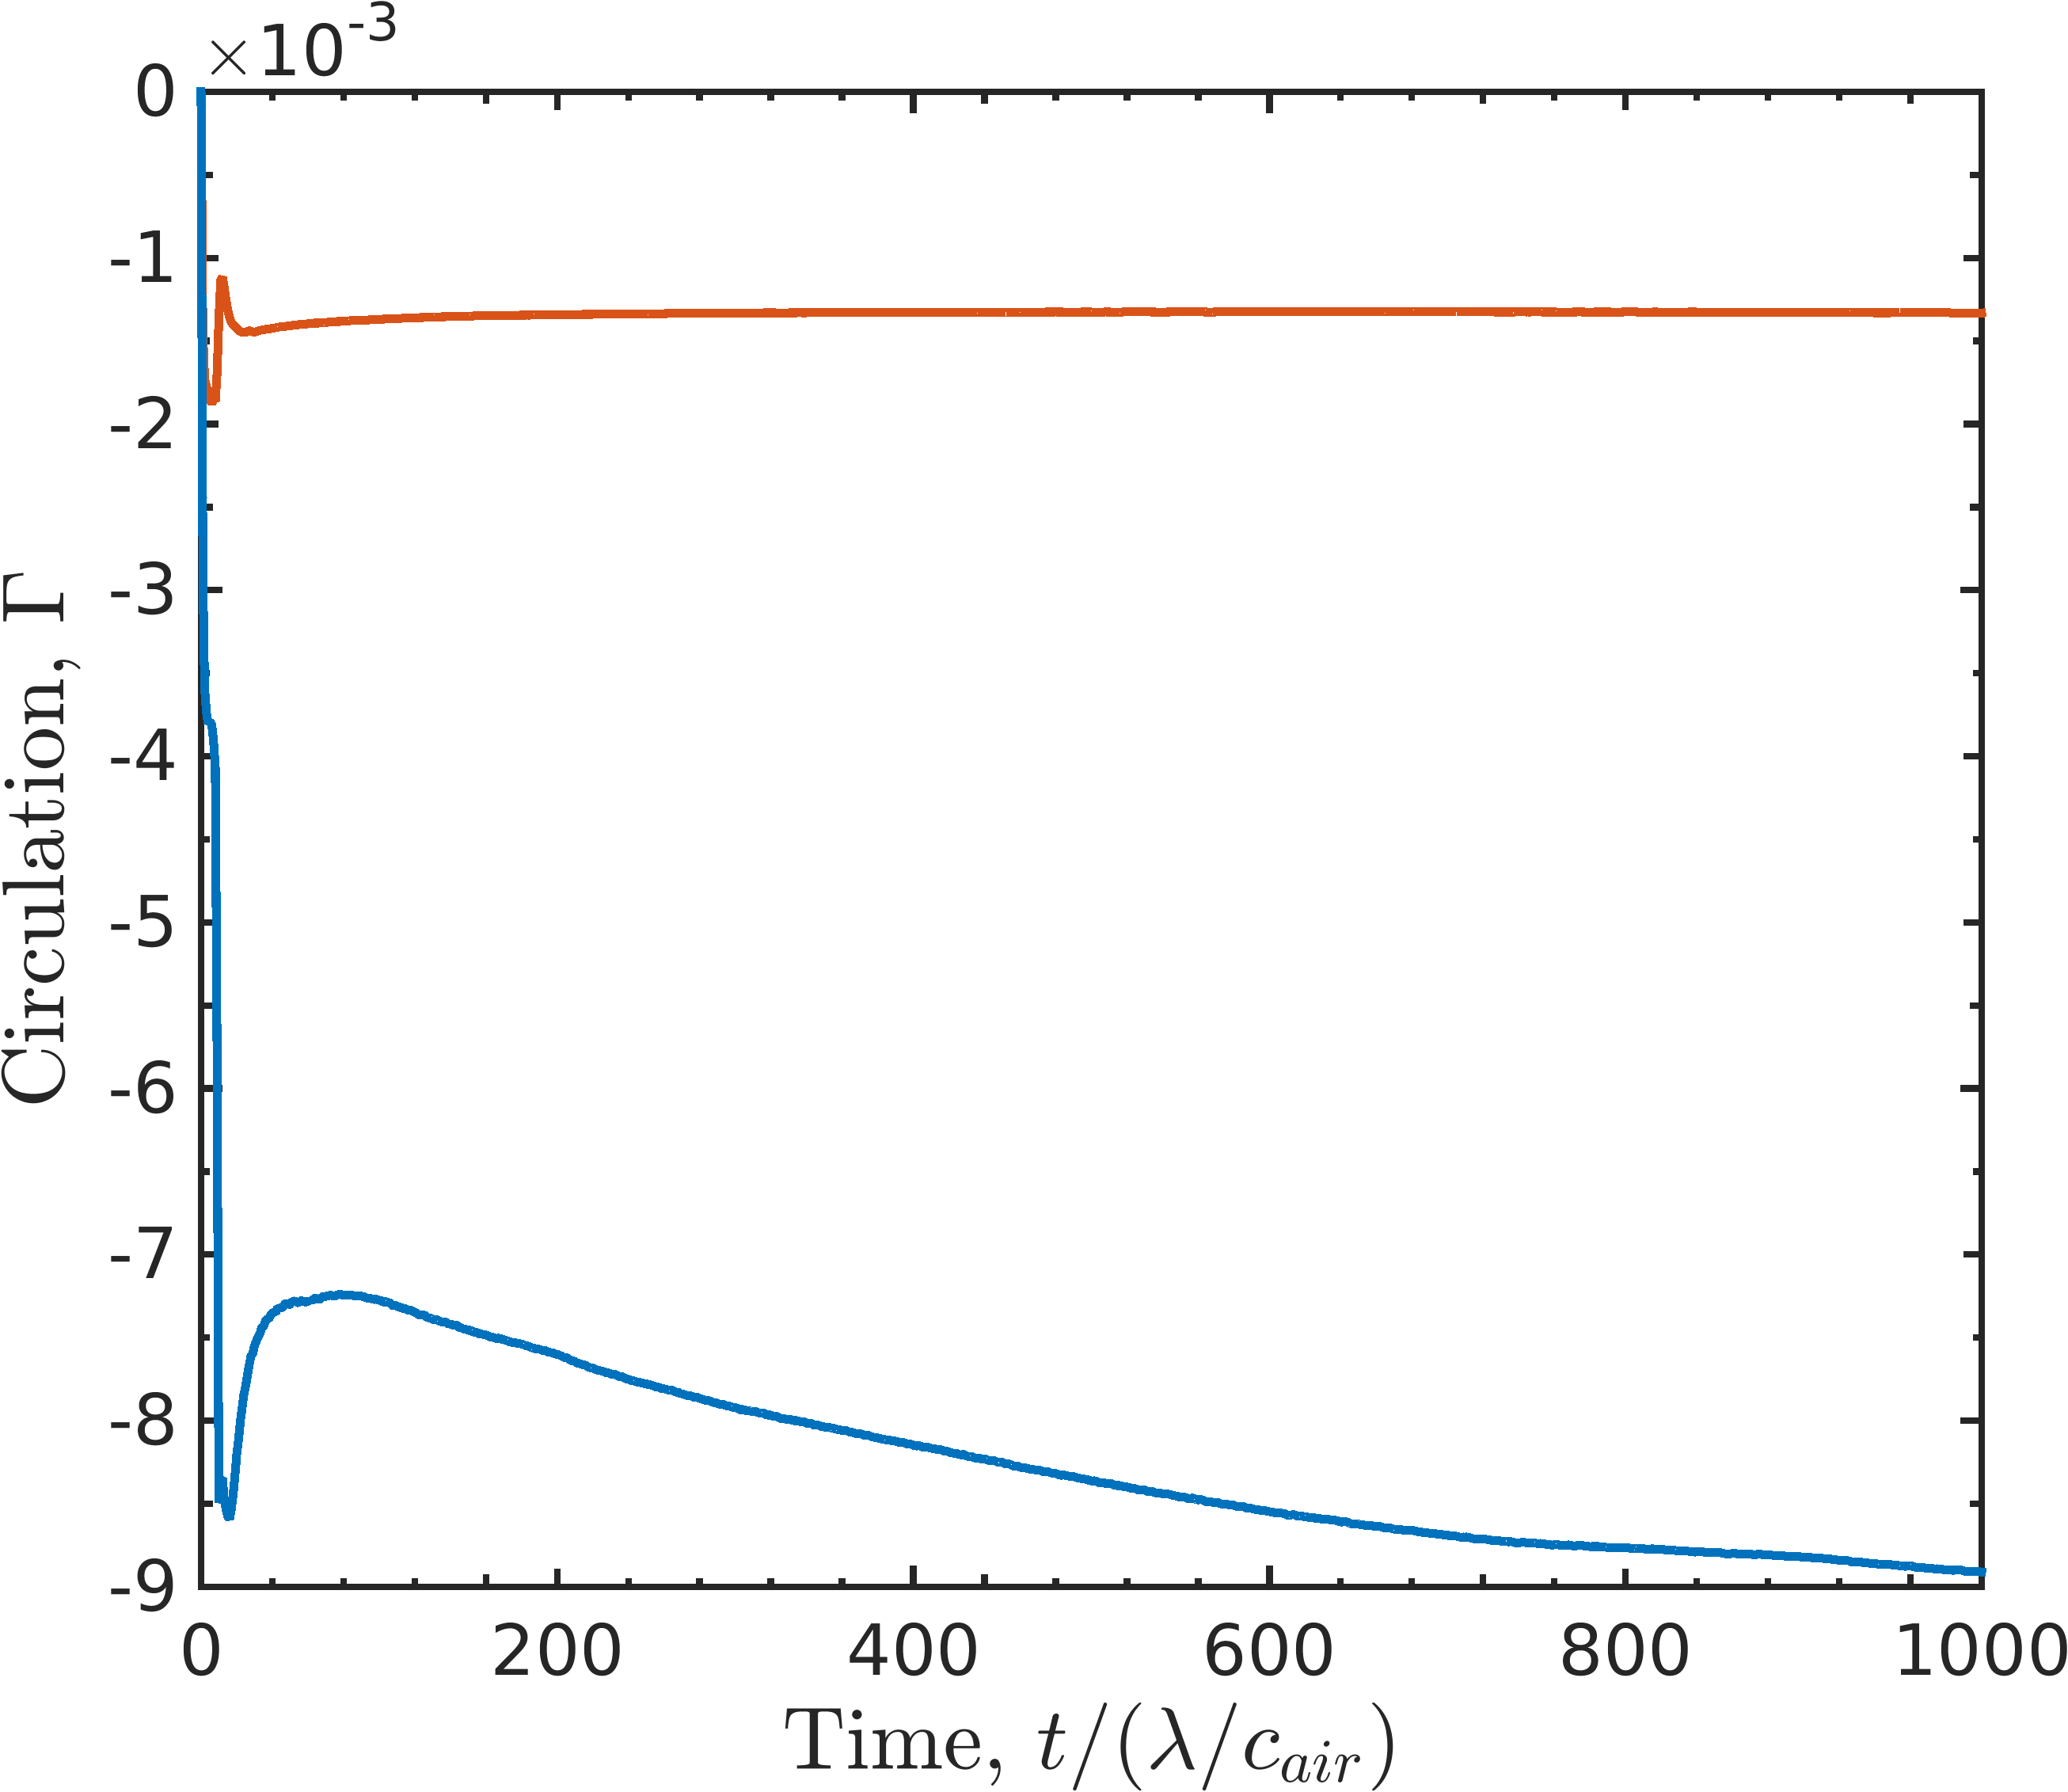
\includegraphics[height=0.45\textheight]{../figs/lung_figs/circulation_multi-amp_roe_t1000}%
    \hfill%
  \end{figure}
  % 
  {\small
    \begin{itemize}
    \item Explain the discrepancies between numerical results and $a(t)\sim\sqrt{\Gamma t}$%
      \vspace*{5pt}
    \item Develop a model and scaling law for circulation
      $\Gamma(\nabla p, a_0)$ deposited on a slightly perturbed
      interface by a compression or expansion wave \vspace*{5pt}
      % \item Develop a model to predict the interface phase-reversal time for a compression wave
      %   \vspace*{5pt}
      % \item Design an acoustic waveform to minimize circulation and interface growth.
      %   \vspace*{5pt}
    \item Invert the waves to confirm counter rotating vertices relevant growth
    \end{itemize}
  }
  \note{
    {\footnotesize
      \begin{enumerate}
      \item Most of the fluids work that I plan to do to increase the
        understanding of the fluid mechanics has been wrapped up, but
        there are a few points that I would like to address over the
        next few months.
      \item I want to explain the discrepancies between our scaling law
        for circulation driven growth and our computational results
        which grow slightly faster.
      \item I want to develop a model and scaling law to describe circulation deposition at the interface.
      \item This will require a few more runs at a few different
        amplitudes, that are currently in place now, but each of these
        runs takes about a month to perform and process.
      \item I've started work on the model, and am assuming a static
        interface, during the short interaction, which isn't too far off
        of what we saw. And am developing ways to express the baroclinic
        vorticity generation term based on the initial pressure wave and
        geometry condition.
      \item If I can get these two things accomplished, we should be
        able to gain insight into the late-time interface growth based
        on the initial conditions for studied regime.
      \item To confirm our current hypothesis of the driving mechanism,
        if we invert the pressure waves used, then we should see
        counter-rotating vorticies to what we see now, and the growth
        should occur in the opposite direction.
      \end{enumerate}
    }
  }
\end{frame}
% 
%%% Local Variables:
%%% mode: latex
%%% TeX-master: "../main"
%%% End:
